\section{Обзор на разгледаните метрики}
В тази глава ще представим основните свойства на разгледаните от нас метрики. Както споменахме вече, ще се фокусираме върху пространства, описващи компактни обекти които \emph{не} притежават хоризонти на събитията. Специално внимание ще отделим върху характерните орбити в тези пространства. По-конкретно ще разгледаме:\\

\noindent\textbf{1) Природата на фотонните орбити.} Те са главния определящ фактор в оптичната проява на тези обекти, понеже те генерират \emph{сянката}.\newline

\noindent\textbf{2) Последните стабилни орбити на масивни частици.} Те са от съществено значение, понеже до голяма степен определят региона на съществуване на равновесна излъчваща среда, което също има директен ефект върху наблюдателните прояви на тези обекти.
 
\subsection{Пространствено-времеви тунели}
За обща дефиниция на пространствено-времеви тунел можем да приемем следното (CIТE VISSER HERE):\\

\emph{Всеки компактен регион от пространство-времето, който притежава топологично проста граница, но топологично нетривиален обем.}\\\newline
Тълкуването на тази дефиниция е следната: Подобно пространство-време притежава свойството да "свързва"$\,$ два отдалечени (потенциално причинно откъснати) региона. Топологично простата граница в горната дефиниция тогава изразява факта, че тези структури са локализирани така, че самото пространство-време е асимптотически плоско. Топологично нетривиалният обем изразява факта, че за да се "свържат"$\,$ два далечни региона, пространството \emph{трябва} да е неедносвързано. Подобни структури за пръв път са били обсъдени в литературата скоро след откриването на решението на Шварцшилд\footnote{ Още през 1916 г. Людвиг Флам CITE показва, че в решението на Шварцшилд може да се намери "втори регион"$\,$ (в последствие, с въвеждането на координати на Крускал, наречен бяла дупка), свързан със самата черна дупка чрез "мост". Тази идея е повдигната отново едва през 1935 г. от Айнщайн и Розен CITE, които преоткриват тази структура, и тя става известна като мост на Айнщайн-Розен. В последствие Фюлер и Уилър CITE показват, че този мост \emph{не} може да бъде прекосен. Може да се покаже, че тази структура е координатен (при това динамичен!) артефакт - за по-подробна дискусия насочваме читателя към CITE HERE.}. Тези първоначални разглеждания са описвали т.н. \emph{непроходими тунели} и затова са предизвикали особен теоретичен интерес. Едва с появата на влиятелната публикация на Морис и Торн CITE MORIS AND THORNE HERE, описваща сферично симетрични \emph{проходими тунели}, тези обекти стават релевантни в теоретичната астрофизика.\newpage

Описването на проходими тунели представлява до голяма степен "обратна задача"$\,$ на решаването на уравненията на Айнщайн-Хилбърт. Започва се с постулат на желаните от обекта свойства и анзац за метриката, удовлетворяващ тези свойства, след което той се замества в полевите уравнения за да се установи типът материя, нужен за поддържане на обекта. Анзацът, който ще използваме, e предложен от Тео CITE TEO HERE като обобщение на резултатите на CITE MORIS AND THORN HERE за \emph{въртящия се случай} е:
	
\begin{equation}
	ds^2 = -N^2(r,\theta)dt^2 + \frac{dr^2}{1 - \frac{b(r,\theta)}{r}} + r^2K^2(r,\theta)\left[d\theta^2 + \sin^2\theta\left(d\phi + \omega(r,\theta)dt\right)^2\right].
\end{equation}
Функциите $N(r,\theta)$ и $\omega(r,\theta)$ са добре известни от 3+1 формулировката на ОТО като функция на времевия поток (lapse function) и на отместването (shift function), докато $b(r,\theta)$ е специфична за тунелите и се нарича функция на формата. Следвайки CITE MORIS AND THORNE HERE, най-общите изисквания към проходим тунел са:\\

\noindent\textbf{1) Липса на хоризонт на събитията.} Метричният анзац (5.1), бивайки аксиално симетричен, притежава вектор на Килинг от вида $k^\mu = \delta_t^\mu + \omega_0\delta^\mu_\phi$, където $\omega_0 = -\frac{g_{t\phi}}{g_{\phi\phi}}$\footnote{Величината $\omega_0$ представлява ъгловата скорост на т.н. \emph{локално невъртящ се наблюдател}. За него имаме, че моментът на импулса му $L_z$ e равен на 0. В аксиално-симетрични пространства от това следва:
	\begin{equation*}
		L_z = k_\phi = g_{\phi\phi}\frac{d\phi}{d\lambda} + g_{t\phi}\frac{dt}{d\lambda} = 0\rightarrow \frac{d\phi}{dt} = -\frac{g_{t\phi}}{g_{\phi\phi}} := \omega_0.
	\end{equation*}
	Ненулевата стойност на $\omega_0$ e проявление на т.н. \emph{eфект на увличане на инерциалните наблюдатели}, породен от смесеният член $g_{t\phi}$ (т.е. от въртенето на централният обект).}. В този случай можем да дефинираме еднозначно хоризонт на събитията като повърхнина, върху която е изпълнено условието $k_\mu k^\mu = 0$. Тогава изискването за липса на хоризонт на събитията е еквивалентно на:

\begin{equation}
g_{\mu\nu} (\delta_t^\mu + \omega_0\delta^\mu_\phi) (\delta_t^\nu + \omega_0\delta^\nu_\phi) \ne 0 \rightarrow g_{tt} - \frac{g_{t\phi}^2}{g_{\phi\phi}} \ne 0.
\end{equation}\newline
Ако презапишем анзацът (5.1) чрез компонентите $g_{\mu\nu}$ виждаме, че тя има вида:
\begin{equation}
	ds^2 = \left(g_{tt} - \frac{g_{t\phi}^2}{g_{\phi\phi}}\right)dt^2 + g_{rr}dr^2 + g_{\theta\theta}d\theta^2 + g_{\phi\phi}\left(d\phi + \frac{g_{t\phi}}{g_{\phi\phi}}d\phi\right)^2.
\end{equation}
Това ни показва, че условието (5.2) е еквивалентно на $N(r,\theta)\ne 0\quad \forall r\in\mathcal{D}_r,\,\forall \theta\in[0,\pi]$, където $\mathcal{D}_r$ е дефиниционното множество на радиалната координата, което ще бъде коментирано в условие 3). За да запази пространството (5.3) своята Лоренцова сигнатура обаче, ние ще наложим условието $N(r,\theta) > 0$. Тогава е удобно да представим $N(r,\theta)$ като:
\begin{equation}
	N(r,\theta) \equiv e^{\Phi(r,\theta)}, \quad |\Phi(r,\theta)| < \infty,\,\, \forall r\in\mathcal{D}_r,\,\,\forall\theta\in[0,\pi]
\end{equation}

\noindent\textbf{2) Асимптотическа плоскост.} Това условие идва от общото физическо съображение, че всеки компактен обект, представляващ локално сгъстяване на материя, не бива да упражнява гравитационно влияние на безкрайност. Това налага следните условия върху метричните функции:

\begin{equation}
	\begin{aligned}
		&N(r,\theta) \xrightarrow[r\rightarrow\infty]{} 1 - \frac{A}{r},\quad \frac{b(r,\theta)}{r} \xrightarrow[r\rightarrow\infty]{} \frac{B}{r} \\
		&\omega(r,\theta)\xrightarrow[r\rightarrow\infty]{} \frac{C}{r^3}\quad\qquad  K(r,\theta) \xrightarrow[r\rightarrow\infty]{} 1,
	\end{aligned}
\end{equation}
където $A$, $B$ и $C$ са константи.

\noindent\textbf{3) Метриката притежава топологията на "тунел".} Това означава, че радиалната координата е ограничена отдолу до минималното разстояние $r_0(\theta)$ такова, че: $1 - \frac{b(r_0,\theta)}{r_0} \ge 0 ,\,\,\forall r\in \mathcal{D}_r = [r_0(\theta),\infty],\,\,\forall\theta\in[0,\pi]$\footnote{Това ограничение върху минималната стойност на радиалната координата има за цел да запази Лоренцовата сигнатура на метриката в цялото пространство.}. За да покажем защо това условие реализира топологията на "тунел"$,$ нека вложим сечението $t = \text{const},\,\,\theta = \text{const}$ на пространството (5.1) в $\mathcal{R}^3$. Линейният елемент тогава заема формата:
\begin{equation}
	ds^2 = \frac{dr^2}{1 - \frac{b(r,\theta)}{r}} + r^2K^2(r,\theta)\sin^2\theta d\phi^2 = \frac{d\rho^2}{1 - \frac{\beta(\rho,\theta)}{\rho}} + \rho^2(\theta)d\phi^2,
\end{equation}
където сме въвели новата координата $\rho = rK(r,\theta)\sin\theta$. Приравняваме (5.6) към линейният елемент на $\mathcal{R}^3$ в цилиндрични координати:
\begin{equation}
	ds^2_{\mathcal{R}^3} = d\rho^2 + \rho^2d\phi^2 + dz^2 = \left[1 + \left(\frac{dz}{d\rho}\right)^2\right]d\rho^2 + \rho^2d\phi^2.
\end{equation}
Идеята на това влагане е да използваме координатата $z$ за визуализиране на тунелната структура. Приравнявайки (5.6) и (5.7) получаваме следното уравнение:
\begin{equation}
	\frac{dz}{d\rho} = \pm \left(\frac{\rho}{\beta(\rho,\theta)} - 1\right)^{-1/2}.
\end{equation}
Кривата $z(\rho,\theta)$ се нарича \emph{функция на влагането}. Виждаме, че за да е реална функция е нужно да бъде изпълнено условието $\frac{\rho(r)}{\beta(\rho(r),\theta)}-1\ge 0$. Равенството дефинира т.н. \emph{гърловина} на тунела $r_0(\theta)$, която играе ролята на долната граница на радиалната координата, спомената по-горе.\\

\noindent За илюстрация нека решим уравнението на влагането (5.8) за $b(r,\theta) = \text{const} = b_0$ и $K(r,\theta) = 1$. Получаваме $z(r) = \pm 2b_0\sqrt{\frac{r}{b_0} - 1}$. Това решение е начертано на фигура \ref{WH_embedding}. Забелязваме, че разходимостта на (5.8) върху гърловината e нужна за формирането на "тунел"$\,$ между регионите, белязани като $I$ и $II$, зависещ от функционалната форма на $b(r)$. Именно оттук следва наименуването ѝ като "функция на формата". Съществуването на реални решения на (5.8) обаче, не е достатъчно да гарантира топология, която свързва две далечни области. Нужно е допълнително условие гласящо, че кривата, описвана от $z(\rho)$, трябва да се "отваря навън"$\,$ от гърловината (т.н. flare out condition). Математически това се изразява в изискването CITE TEO HERE:
\begin{equation}
	\frac{d^2\rho}{dz^2}\bigg\vert_{r = r_0(\theta)} > 0\rightarrow \frac{b(r,\theta) - r\partial_rb(r,\theta)}{2b^2(r,\theta)}\bigg\vert_{r = r_0(\theta)} > 0.
\end{equation}\newline

\noindent\begin{minipage}{15em}
	\centering
	\hspace{-0.99cm}
	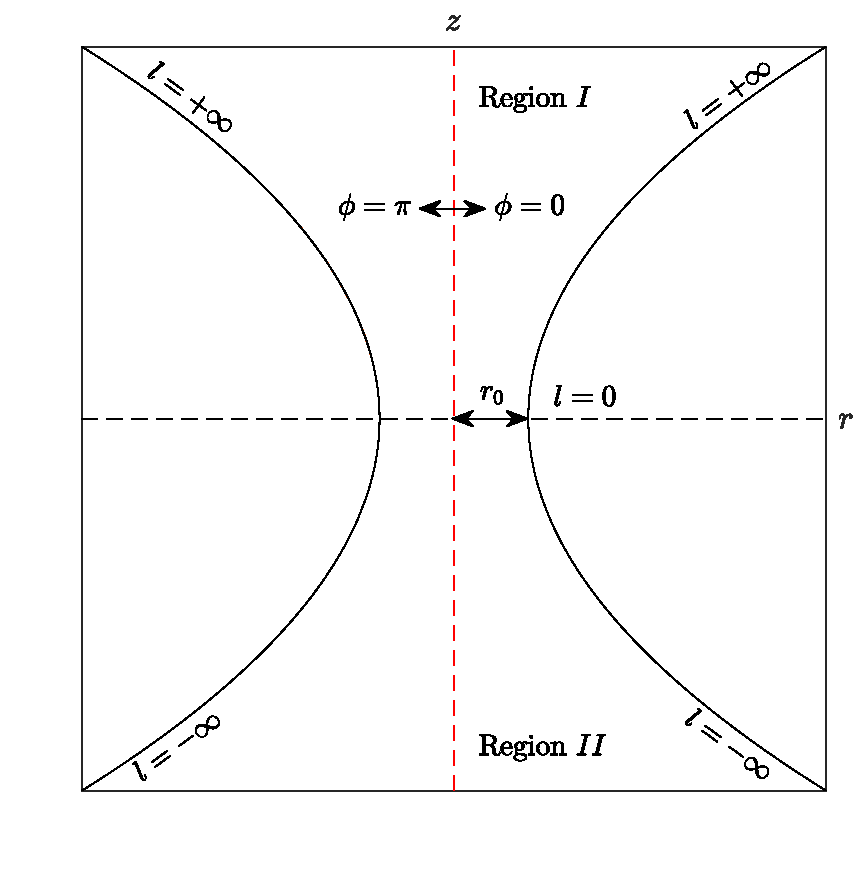
\includegraphics[scale = 0.4]{WH_embedding.pdf}
	\captionof{figure}[Влагаща диаграма на пространствено-времеви тунел]{\small Влагаща диаграма на пространствено-времеви тунел за частният случай на $b(r,\theta) = \text{const} = b_0$}
	\label{WH_embedding}
\end{minipage}\,\,
\begin{minipage}{20em}
	Можем да забележим обаче, линейният елемент (5.1) притежава сингулярност върху гърловината $r_0(\theta) = b(r_0,\theta)$. Подобно на координатната сингулярност в решението на Шварцшилд при $r = 2M$, тя може да бъде отстранена с подходяща смяна на координатите 
	\begin{equation}
	r	 \rightarrow \ell^2(r,\theta) = r^2 - b^2(r,\theta).
	\end{equation}
	
	Тогава разходящият член от (5.1) се превръща в:
	\begin{equation}
		\frac{dr^2}{1 - \frac{b(r,\theta)}{r}} \rightarrow \left[1 + \frac{b(r,\theta)}{r}\right]d\ell^2
	\end{equation}
	
\end{minipage}\\\newline
Координатата $\ell(r,\theta)$ се нарича \emph{глобална}, понеже позволява гладко преминаване през гърловината на тунела. Условно идентифицираме региона с $\ell >0$ като "нашата"$\,$ страна на тунела, докато този с $\ell < 0$ като "другата"$\,$ страна.\\

\noindent\textbf{4) Липса на физически сингулярности.} Пресмятайки скалара на Ричи $R$, може да се покаже, че той има следната форма върху гърловината $r_0(\theta) = b(r_0,\theta)$ CITE HRE:
\begin{equation}
	\begin{aligned}
		(rK)^2R = &-\frac{3}{2}\frac{(\partial_\theta b)^2}{(r - b)^2} - \frac{\partial^2_\theta b}{r - b}
	- \frac{2}{r^2K^2}\left[\partial_\theta \Phi + \frac{\partial_\theta K}{K} + \frac{\partial_\theta b}{r}\right]\cot\theta + \\ 
	& + \text{reg. terms}.
	\end{aligned}
\end{equation}

\noindent Виждаме, че за избегнем сингулярности върху оста на въртене $\theta = 0,\pi$, e нужно да занулим следните членове върху гърловината:

\begin{equation}
	\partial_\theta \Phi(r_0(\theta),\theta) = 0\big\vert_{\theta = 0,\pi},\, \partial_\theta K(r_0(\theta),\theta)\big\vert_{\theta = 0,\pi} = 0,\,\partial_\theta b(r_0(\theta),\theta)\big\vert_{\theta = 0,\pi} = 0.
\end{equation}
Докато за да избегнем сингулярности върху самата гърловина е нужно да наложим:
\begin{equation}
	\partial_\theta b(r,\theta)\big\vert_{r = r_0} = 0,\, \partial^2_\theta b(r,\theta)\big\vert_{r = r_0} = 0.
\end{equation}
Можем да видим, че частният случай от фигура \ref{WH_embedding} изпълнява всички тези условия.\\

\noindent\textbf{Вече можем да запишем конкретната форма на анзацa (5.1) използван от нас:}
\begin{equation}
	N(r,\theta) = e^{-\frac{r_0}{r} - \gamma\frac{r_0^2}{r^2}},\, b(r,\theta) = r_0,\, K(r,\theta) = 1,\, \omega(r,\theta) = \frac{2a}{r^3}
\end{equation}

\subsubsection{Физическа интерпретация на параметрите на тунела}

Понеже методиката за построяване на решение, описващо тунел в пространство-времето, не започва с постулирането на разпределение от материя, е нужно специално внимание за интерпретирането на параметрите в развитието (5.5).\\

\noindent\textbf{Интерпретация на константата $B$.} Нейната стойност зависи директно от асимптотичното поведение на функцията на формата и следователно няма обща физическа интерпретация сама по себе си (още повече след като имаме свободата да избираме природата на $b(r,\theta)$, стига тя да удовлетворява свойствата (5.13) и (5.14)). По-скоро на нея трябва да се гледа като условие върху тензора на момента и импулса, и следователно върху материята която генерира тунела.\\

\noindent\textbf{Интерпретация на константата $A$.} Понеже разглежданият общ анзац (5.1) е статичен, можем да пресметнем за него интегралите на Комар. По-конкретно нека пресметнем \emph{масата на Комар} $M_{\text{Komar}}$. Тя се задава с израза:
\begin{equation}
	M_{\text{Komar}} = -\frac{1}{4\pi}\int_{\partial\Sigma}\nabla^\mu k^\nu_t dS_{\mu\nu} =  -\frac{1}{4\pi}\int_{\partial\Sigma}\nabla^\mu k^\nu_t\left[n_\mu\sigma_\nu - n_\nu\sigma_\mu\right] \sqrt{\sigma}d^2y,
\end{equation}
където $k^\mu_t = (-1,0,0,0)$ и интегралите са по границата на времеподобно 3-мерно многообразие $\Sigma_t$, дефинирано като $\mathcal{M} = \mathcal{R} \times \Sigma_t$. Т.е. $\Sigma_t$ представлява пространственото сечение на $\mathcal{M}$ за фиксирано координатно време $t$. Може да се покаже, че (5.15) не зависи от избора $\Sigma_t$, поради което индексът е изпуснат. Тогава можем да интерпретираме $\partial\Sigma$ като пространствена безкрайност $r\rightarrow\infty$ и $\sqrt{\sigma}$ като индуцирана метрика върху 2-мерната сфера $r = \text{const}, t = \text{const}$. Векторите $n_\mu = - (\sqrt{-g_{tt}}, 0, 0, 0)$ и $\sigma_\nu = (0, \sqrt{g_{rr}},0 ,0)$ представляват нормалите на $\Sigma$ и $\partial\Sigma$. Пресмятайки израза (5.16), използвайки анзацa (5.15), получаваме следния резултат REF APENDIX HERE:
\begin{equation}
	M_{\text{Komar}} = r_0 \xrightarrow[(5.15)]{} A = M_{\text{Komar}}
\end{equation}

\noindent\textbf{Интерпретация на константата $C$.} Нека сега пресметнем \emph{момента на импулса на Комар} $J_{\text{Komar}}$, дефиниран като:
\begin{equation}
	J_{\text{Komar}} = \frac{1}{8\pi}\int_{\partial\Sigma}\nabla^\mu k^\nu_\phi dS_{\mu\nu} = \frac{1}{8\pi}\int_{\partial\Sigma}\nabla^\mu k^\nu_\phi\left[n_\mu\sigma_\nu - n_\nu\sigma_\mu\right] \sqrt{\sigma}d^2y,
\end{equation}
където $k^\phi = (0, 0, 0, 1)$. Отново, самото изчисление може да се намери в REF APENDIX HERE, крайният резултат е следният:
\begin{equation}
	J_\text{Komar} = a\xrightarrow[(5.15)]{} C = 2J_\text{Komar}, 
\end{equation}
където $a$ представлява нормирания момент на импулса на тунела.
\subsubsection{Оптична проява - фотонни орбити и сенки}
Нека сега разгледаме динамичните уравнения на фотоните в пространство-времето на тунела. Както вече споменахме в Глава 2, свойствата на тези уравнения еднозначно определят видимата форма на обекта на небето.\\

\noindent Отчитайки чистата радиална зависимост на функциите (5.15) и замествайки явната форма на метриката (5.1) в уравнението на Хамилтон-Якоби, извършваме разделянето на променливите за да стигнем до следната система от динамични уравнения:
\begin{subequations}
	\begin{equation}
		\frac{dt}{d\lambda} = \frac{E - \omega(r)L_z}{N^2(r)}
	\end{equation}
	\begin{equation}
		\frac{N(r)}{\sqrt{1 - \frac{b(r)}{r}}}\frac{dr}{d\lambda} = \pm \sqrt{R(r)}
	\end{equation}
	\begin{equation}
		r^2K^2(r)\frac{d\theta}{d\lambda} = \pm \sqrt{\Theta(\theta)}
	\end{equation}
	\begin{equation}
		\frac{d\phi}{d\lambda} = \omega(r)\frac{E - \omega(r)L_z}{N^2(r)} + \frac{L_z}{r^2K^2(r)\sin^2\theta},
	\end{equation}
\end{subequations}
където потенциалите $R(r)$ и $\Theta(\theta)$ се задават от функциите:
\begin{subequations}
	\begin{equation}
		R(r) = -C\frac{N^2(r)}{r^2K^2(r)} + (E - \omega(r)L_z)^2 - m^2N^2(r)\\
	\end{equation}
	\begin{equation}
		\Theta(\theta) = C - \frac{L_z^2}{\sin^2\theta}
	\end{equation}
\end{subequations}
и $C = k_\theta^2 + \frac{L_z^2}{\sin^2\theta}$ е константата на Картер.
Може да отбележим някои неща за тази система:\\

\noindent\textbf{1)} Тя е валидна когато всички метрични функции в (5.1) имат само радиална зависимост. Това представлява по-общ случай, който обхваща и нашия конкретен избор на функции (5.15).\\

\noindent\textbf{2)} Уравнение (5.20г) има интересното свойство, че по явен начин отделя ефекта на увличане на инерциални наблюдатели (левият член) от "естествената"$\,$ азимутална динамика (десният член). Т.е то има вида $\frac{d\phi}{d\lambda} = g(a,r) + f(r),\,\, g(a = 0, r) = 0$\newpage

Както споменахме вече в глава 2, основен интерес за нас представляват фотонните орбити (поради директната им връзка с видимата форма на обектите на небето). Нека сега използваме системата (5.20) за да намерим условията, при които тези фотони попадат в \emph{нестабилни}\footnote{За разлика от черни дупки на Кер, метриката (5.15) допуска съществуването на \emph{стабилни} фотонни орбити, които обаче нямат принос към сянката. За по-подробна дискусия виж CITE HERE} кръгови орбити около тунела:
\begin{subequations}
	\begin{equation}
	\left(\frac{dr}{d\lambda}\right)^2 = \frac{1}{N^2(r)}\left(1 - \frac{b(r)}{r}\right)R(r) = - V_\text{eff} = 0
	\end{equation}
	\begin{equation}
		\frac{d^2r}{d\lambda^2} = -\frac{1}{2}\frac{dV_{\text{eff}}}{dr} = 0
	\end{equation}
	\begin{equation}
		\frac{d^2V_\text{eff}}{dr^2} \le 0
	\end{equation}
\end{subequations}
Решенията на системата (5.22) могат да се разделят на два класа: такива, намиращи се \emph{извън} гърловината $r_{\text{ph}} > b(r)$, и такива \emph{върху} нея $r_\text{ph} = b(r)$. Нека ги разгледаме поотделно:\\
	
\noindent\textbf{1)} За първия клас имаме, че е изпълнено $1 - \frac{b(r)}{r}ЮС \ne 0$. Следователно системата (5.22) се свежда до:
	\begin{equation}
		R(r) = 0,\,\, \frac{dR(r)}{dr} = 0,\,\, \frac{d^2R(r)}{dr^2} \ge 0
	\end{equation}
	Полагайки $m = 0$ в (5.21а), и въвеждайки означенията $\eta = C / E^2$ и $\xi = L_z / E$, получаваме следната връзка между интегралите на движение на фотоните:
	\begin{subequations}
		\begin{equation}
			\eta = \frac{r^2K^2(r)}{N^2(r)}\left(1 - \omega(r)\xi(r)\right)^2
		\end{equation}
		\begin{equation}
			\xi(r) = \frac{\Sigma(r)}{\Sigma(r)\omega(r) - \frac{d}{dr}\omega(r)},\,\, \Sigma(r) = \frac{d}{dr}\ln\left(\frac{N(r)}{rK(r)}\right)
		\end{equation}
	\end{subequations}

	Изпълняването на тези връзки в екваториалната равнина $\theta = \pi / 2$ дефинира \emph{най-външната} възможна фотонна орбита, която ще бележим като $r_{\text{ph}}^-$. Това е така понеже замествайки връзките (5.24) в потенциала (5.21б), намираме, че той е монотонно намаляваща функция на $r$. На фигура \ref{WH_rph} е представено численото решението за на системата (5.24) за $r^-_{\text{ph}}(a,\gamma)$. \\
	
	\noindent\begin{minipage}{14em}
		\hspace{-0.5cm}
		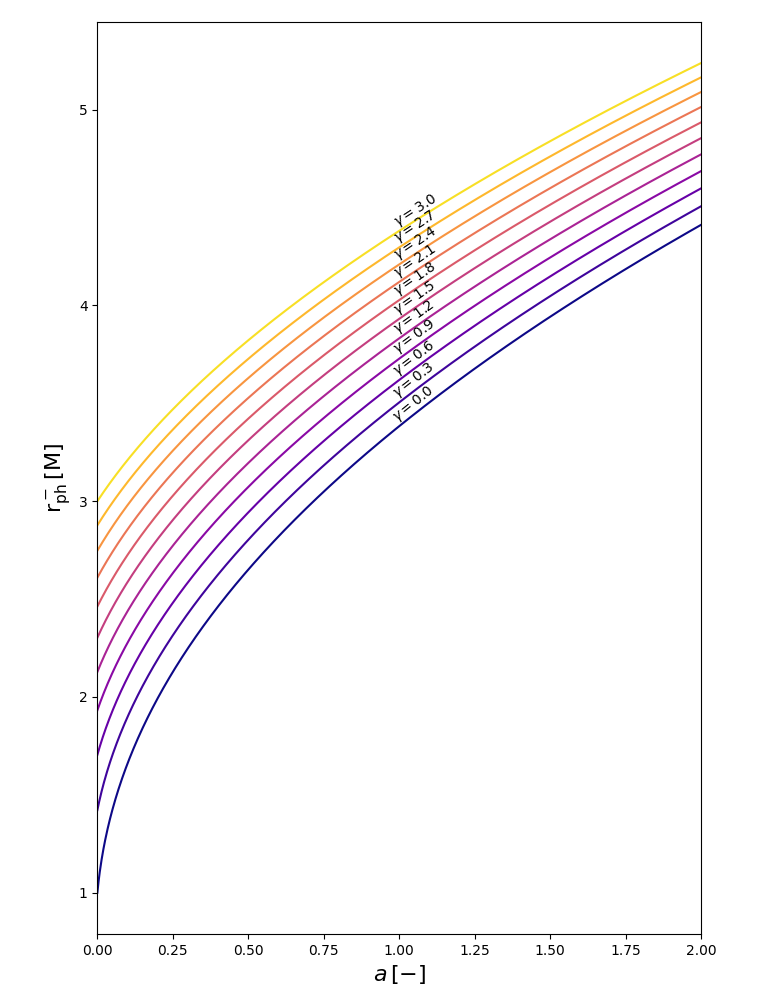
\includegraphics[scale = 0.35]{WH_rph.png}
		\captionof{figure}[Фотонни орбити на пространствено-времеви тунели]{\small Външните фотонни орбити като функция на параметъра на въртене, за избрани стойности на $\gamma$.}
		\label{WH_rph}
	\end{minipage}\,\,\,
	\begin{minipage}{20em}
		Тя притежава аналитично решение за частния случай $a = 0$:
		\begin{equation}
			r^-_\text{ph}(a = 0,\,\gamma) = \frac{r_0}{2}\left(1 + \sqrt{1 + 8\gamma}\right)
		\end{equation}
		Можем да забележим, че произведението $a\xi(r_{\text{ph}}^-)<0$ (от израз (5.24б)). Това означава, че този клас от отбити са \emph{ретроградни}.\\
		
		2) За втория клас имаме, че $r_{\text{ph}} = b(r)$. Тогава системата (5.21) се свежда до следната:
		\begin{equation}
			r = b(r),\,\, R(r) = 0,\,\, \frac{dR(r)}{dr} \ge 0.
		\end{equation}

		Тези условия са еквивалентни на:
		\begin{subequations}
			\begin{equation}
				\eta = \frac{r^2K^2(r)}{N^2(r)}\left(1 - \omega(r)\xi\right)^2\bigg\vert_{r = b(r)}
			\end{equation}
			\begin{equation}
				 \xi_\text{min} = \frac{\Sigma(r)}{\Sigma(r)\omega(r) - \frac{d}{dr}\omega(r)}\bigg\vert_{r = b(r)}
			\end{equation}
			\begin{equation}
				\xi_\text{max} = \frac{r\sin\theta}{N + \omega r \sin\theta}\bigg\vert_{r = b(r),\,\,\theta = \theta_{\text{obs}}}
			\end{equation}
		\end{subequations}

	\end{minipage}\\\newline

Тези два класа орбити дефинират параметрично (чрез интегралите на движение $\xi$ и $\eta$) два отделни сегмента от контура на сянката на тунела. Връзката между изразите (5.24), (5.27) и координатите на този контур върху небето са изведени в Допълнение Б. Тук ще ги запишем за удобство на изложението:
\begin{subequations}
	\begin{equation}
		\alpha = \arctan\left(\frac{\xi}{\bar{k}_r}\sqrt{\frac{g_{rr}}{g_{\phi\phi}}}\right)\bigg\vert_{\vec{r} = \vec{r}_\text{obs}},\,\,\, \bar{k}_r = \frac{k_r}{E} 
	\end{equation}
	\begin{equation}
		\beta = \arcsin\left(\frac{1}{\zeta - \delta \xi}\frac{\bar{k}_\theta}{\sqrt{g_{\theta\theta}}}\right)\bigg\vert_{\vec{r} = \vec{r}_\text{obs}} ,\,\,\, \bar{k}_\theta = \frac{k_\theta}{E} 
	\end{equation}
	\begin{equation}
		\zeta = \sqrt{\frac{g_{\phi\phi}}{g^2_{t\phi}-g_{tt}g_{\phi\phi}}},\,\,\, \delta = - \frac{g_{t\phi}}{g_{\phi\phi}}\zeta\bigg\vert_{\vec{r} = \vec{r}_\text{obs}} .
	\end{equation}
\end{subequations}

Импулсите $k_r$ и $k_\theta$ се задават от динамичните уравнения (5.20). На фигура \ref{WH_shadows} са начертани пълните сенки за някои избрани стойности на метричните параметри $\gamma$ и $a$.\\

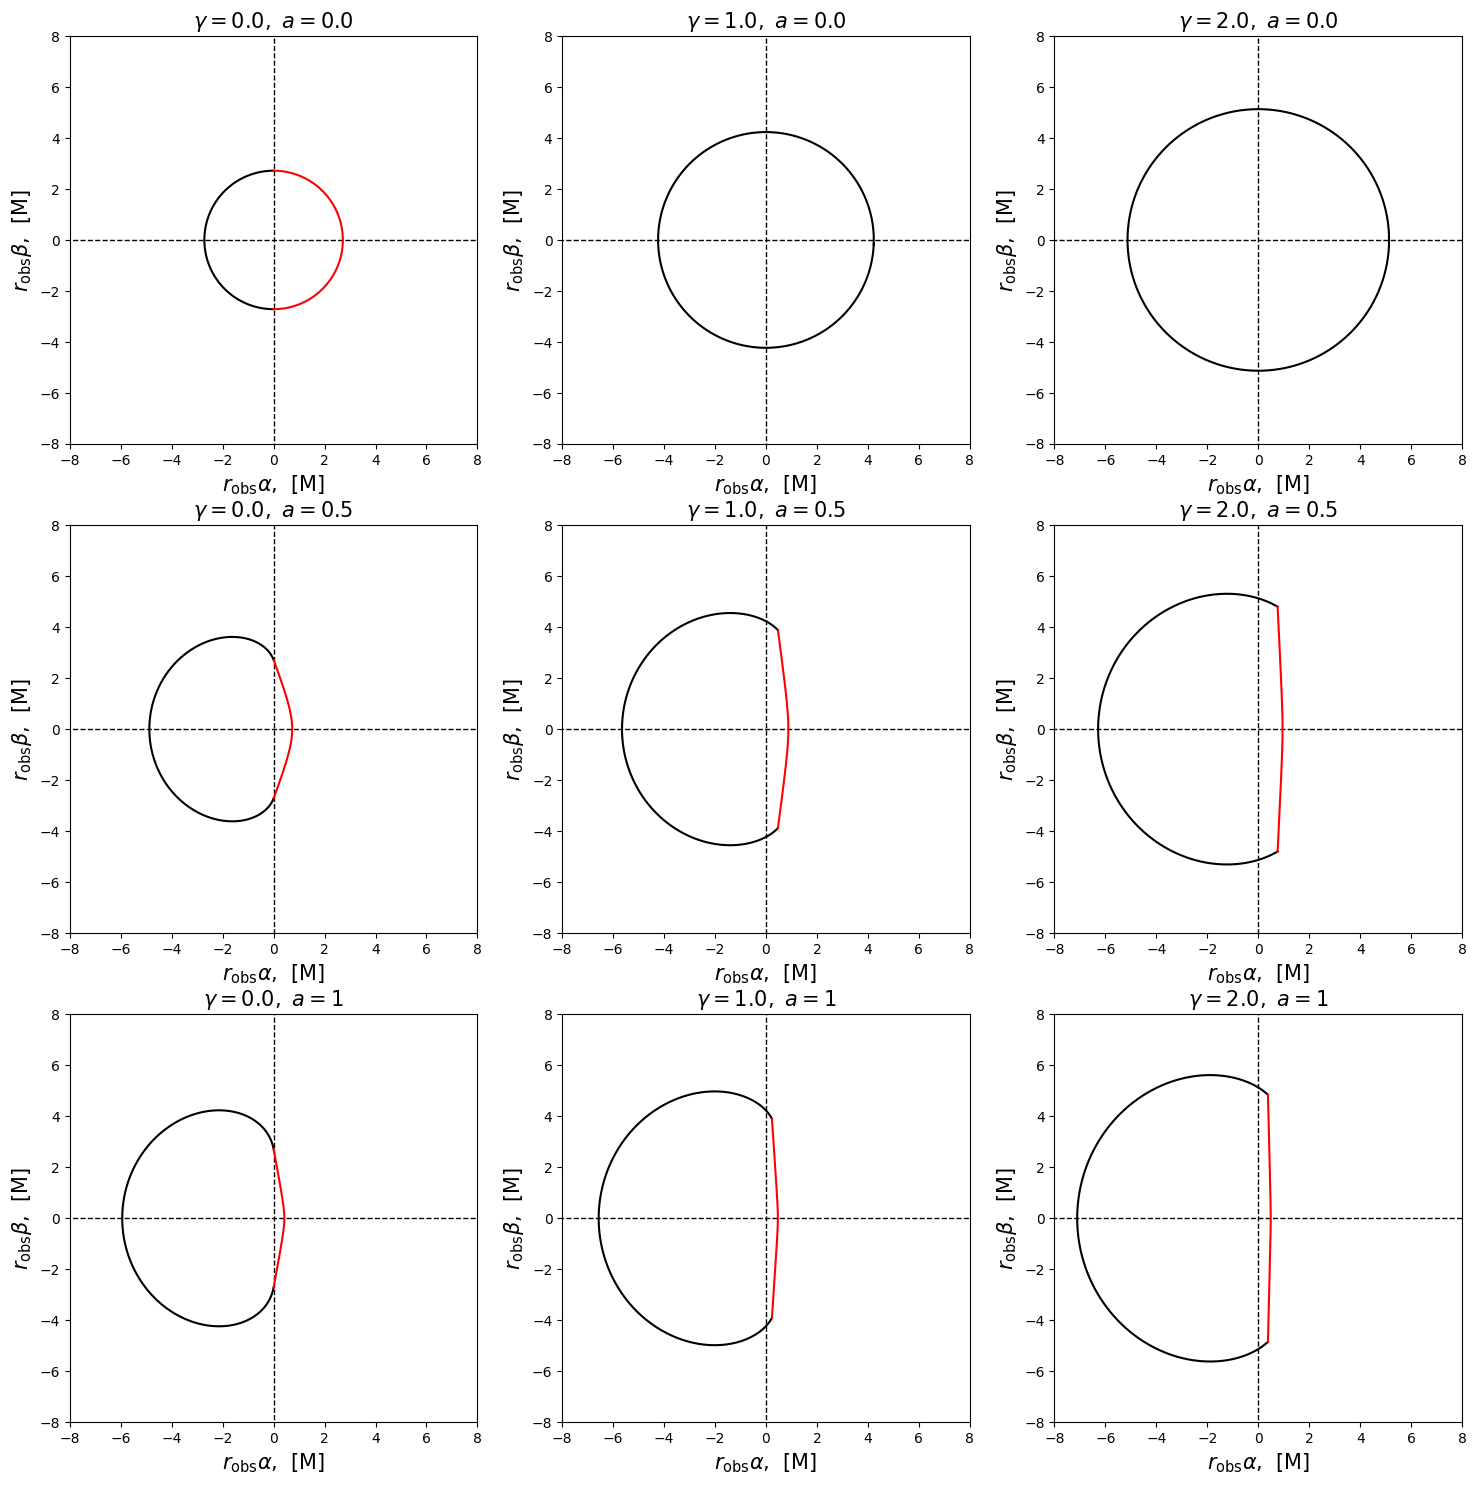
\includegraphics[scale = 0.37]{WH_Shadows.png}
\captionof{figure}[Сенки на пространствено-времеви тунели]{\small Сенките за далечен наблюдател при някои избрани стойности на параметрите $\gamma$ и $a$ при $\theta_\text{obs} = \pi / 2$. Червеният контур съответства на фотонните орбити върху гърловината, докато черният - на тези извън нея. Координатите $\{\alpha,\,\beta\}$ представляват наблюдателните ъгли по небесната сфера.}
\label{WH_shadows}
$\,$
\newline
Забелязваме, че при стационарния случай $a = 0$ (с изключение на $\gamma = 0$), сянката се формира изцяло от фотоните, удовлетворяващи условия (5.24) извън гърловината. Частният случай на $\gamma = a = 0$ се различава с това, че при него орбитите, описвани (5.24) също се намират върху гърловината (както може да видим от (5.25)). Също забелязваме, че морфологията на сянката се мени много бързо с увеличаване на параметъра на въртене $a$ (за разлика от черните дупки на Кер). По-подробна дискусия върху взаимодействието на двата клона на сянката може да се намери в CITE HERE.
\newpage
\subsubsection{Характерни орбити на масивни частици}
Общите разглеждания за екваториални орбити на масивни частици в аксиално симетрични пространства е представено в Допълнение Х. От интерес представляват две конкретни орбити:\\

\textbf{1) Най-вътрешната стабилна кръгова орбита (ISCO)}, дефинирана от условията (виж ДОПЪЛНЕНИЕ):
\begin{subequations}
	\begin{equation}
		\frac{1}{g_{rr}g_2}\left[-\partial_r^2g_{2} + E^2\left(\partial_r^2g_{\phi\phi} + 2\ell\partial_r^2g_{r\phi} + \ell^2\partial_r^2g_{tt} \right)\right] = 0,
	\end{equation}
	където енергията на частиците $E$, специфичният им азимутален момент на импулса $\ell$ и Кеплеровата им орбитална честота $\Omega$ се задават с изразите:
	\begin{equation}
		E(r) = -\frac{g_{tt} + g_{t\phi}\Omega(r)}{\sqrt{-g_{tt} - 2g_{t\phi}\Omega(r) - g_{\phi\phi}\Omega^2(r)}}
	\end{equation}
	\begin{equation}
		\ell(r) = \frac{L_z(r)}{E(r)} = - \frac{g_{\phi\phi}\Omega(r) + g_{t\phi}}{g_{tt} + g_{t\phi}\Omega(r)}
	\end{equation}
	\begin{equation}
		\Omega(r) = -\frac{\partial_rg_{t\phi}}{\partial_rg_{\phi\phi}} \pm \frac{\sqrt{(\partial_rg_{t\phi})^2 - \partial_rg_{tt}\partial_rg_{\phi\phi}}}{\partial_rg_{\phi\phi}},
	\end{equation}
	и метричната функция $g_2$ се дефинира като
	\begin{equation}
		g_2 = g_{t\phi}^2 - g_{tt}g_{\phi\phi}
	\end{equation}
\end{subequations}
Знакът "плюс"$\,$ в израз (5.29г) съответства на движение по посоката на въртене на обекта, докато знакът "минус"$\,$ - обратното. Горната система има точно решение в стационарният случай $a = 0$:
\begin{equation}
	r_{\text{ISCO}}(a = 0, \gamma) = 2M \left[\sqrt{\frac{4}{9}(6\gamma+1)}\cosh\left\{\frac{1}{3}\arccosh\left[\frac{1 + 9\gamma + \frac{27}{2}\gamma^2}{(6\gamma + 1)^{3/2}}\right]\right\} + \frac{1}{3}\right].
\end{equation}
Както при фотонните орбити, и тук имаме два класа решения - върху гърловината $\frac{1}{g_{rr}} = 0$, и такива извън нея $\frac{1}{g_{rr}} \ne 0$ (представени на фигура \ref{WH_ISCO}). Интересна характеристика на тези решенията можем да видим на левия панел. Орбити с посока на движение, съвпадаща с тази на въртенето на тунела, съществуват извън гърловината само за малки стойности на параметъра на въртене $a < a_\text{crit}(\gamma)$. При $a > a_\text{crit}(\gamma)$ тези орбити "падат"$\,$ (прекъснато) върху гърловината. Това свойство и следствията от него ще бъдат коментирани допълнително при разглежданията ни в глава Х.\\

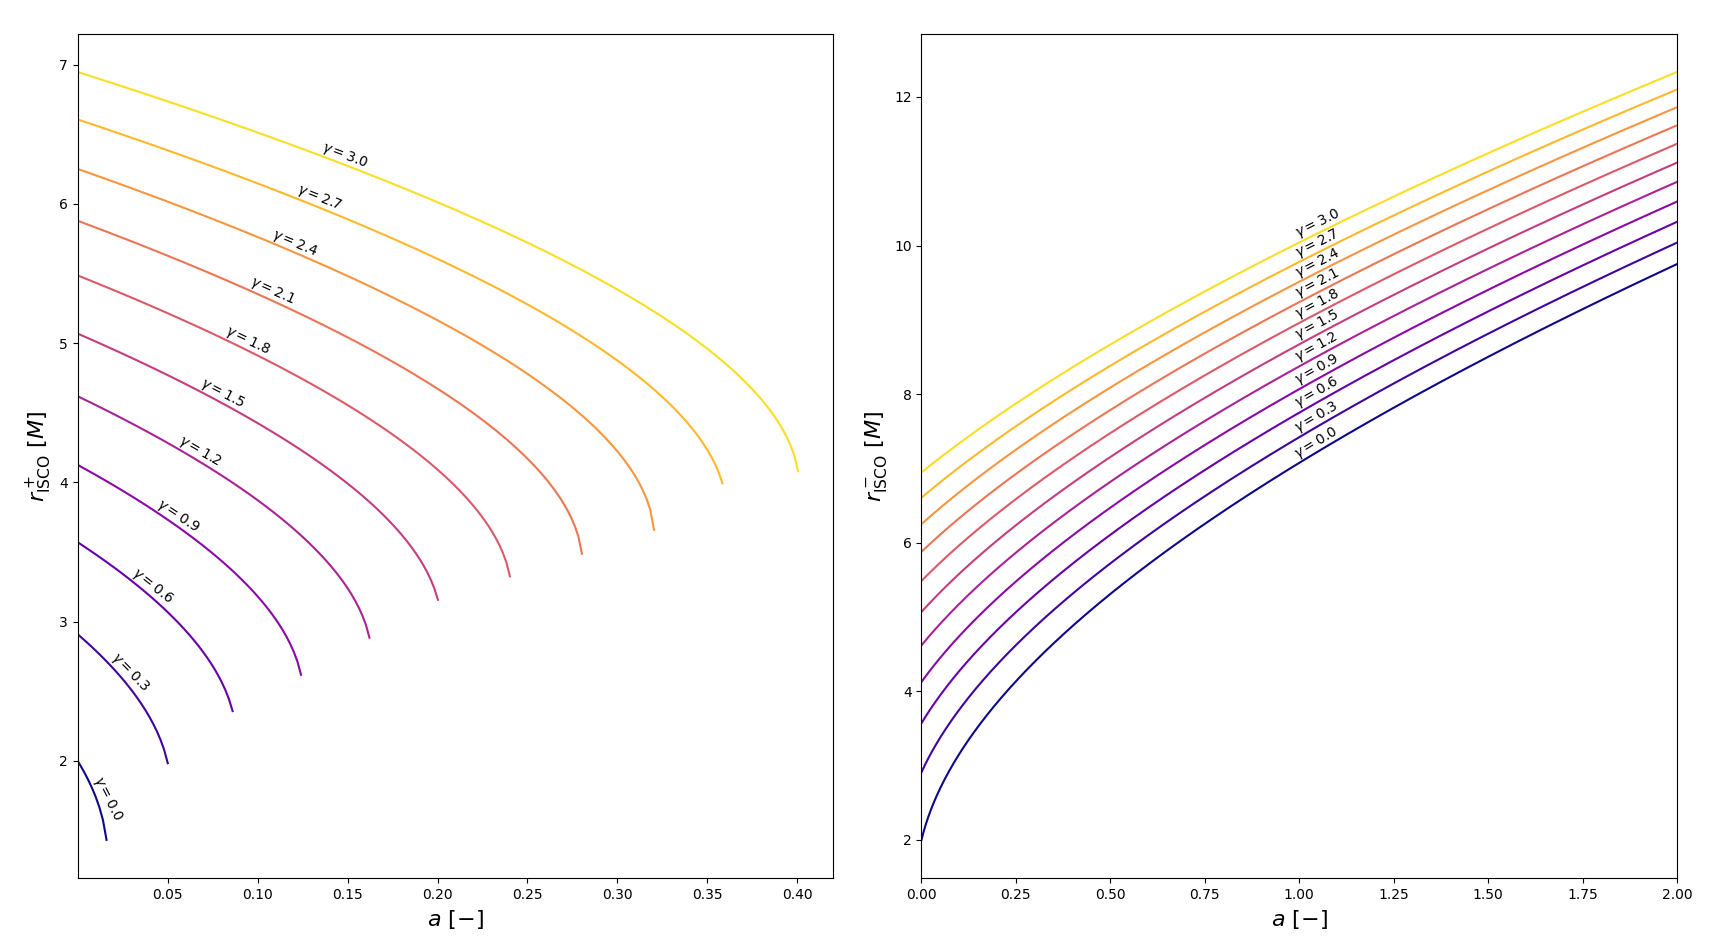
\includegraphics[scale = 0.35]{WH_ISCO.png}
\captionof{figure}[ISCO Орбити за пространствено-времеви тунели]{\small ISCO орбитите като функция на параметъра на въртене $a$ за някой избрани стойности на $\gamma$. Орбитите с движение по посока на въртенето на тунела съществуват извън гърловината само за малки стойности на $a$.}
\label{WH_ISCO}

$ $\newline\textbf{2) Последните свързани орбити}, дефинирани от условието:
\begin{equation}
	E(r) = -\frac{g_{tt} + g_{t\phi}\Omega(r)}{\sqrt{-g_{tt} - 2g_{t\phi}\Omega(r) - g_{\phi\phi}\Omega^2(r)}} = 1
\end{equation}

\hspace{-0.5cm}
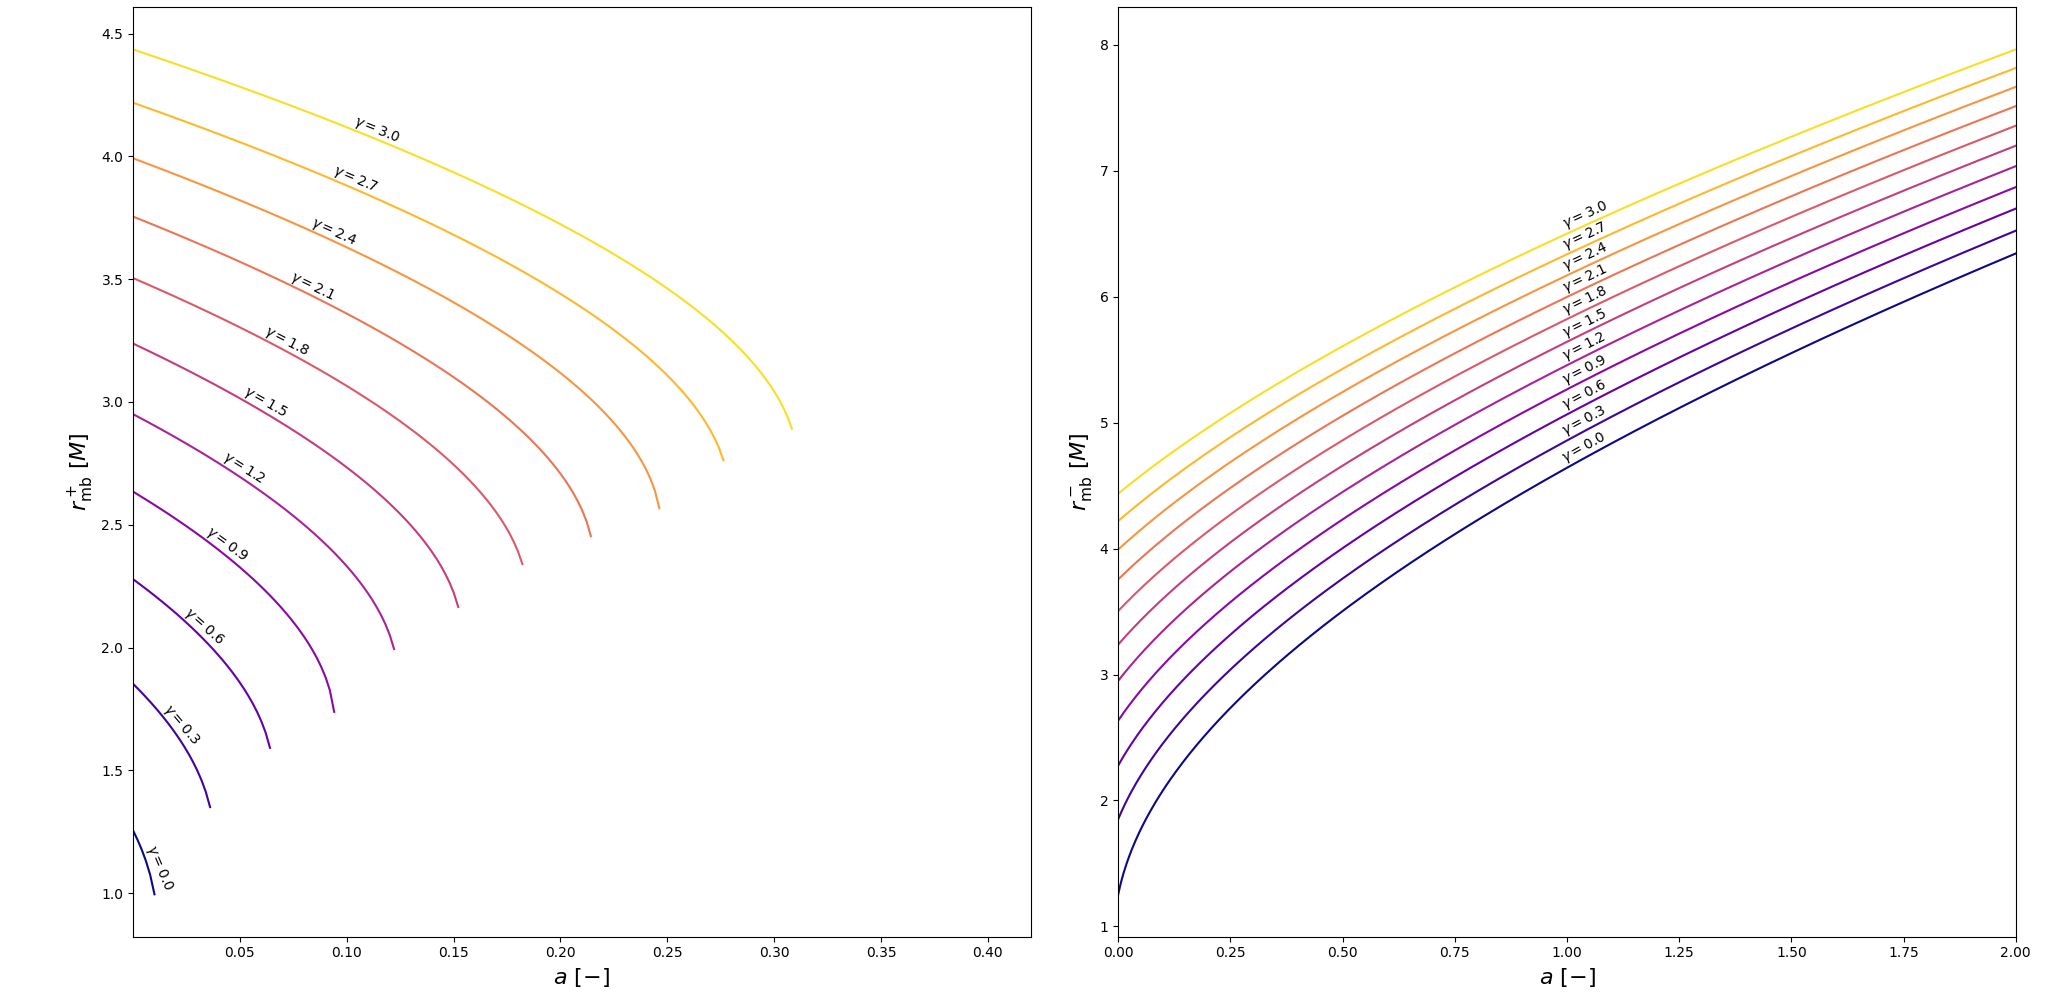
\includegraphics[scale = 0.3]{WH_mb.png}
\captionof{figure}[Последните свързани орбити за пространствено-времеви тунели]{\small Последните свързани орбити като функция на параметъра на въртене $a$ за някои избрани стойности на $\gamma$. Орбитите с движение по посока на въртенето на тунела съществуват извън гърловината само за малки стойности на $a$.}
\label{WH_mb}

\newpage
\subsection{Голи сингуларности на Джанис-Нюман-Уиникър}

Тези обекти, за разлика от пространствено-времевите тунели, са \emph{точни} решения. По-конкретно те представляват най-общите сферично симетрични решения на полевите уравнения на Айнщайн-Хилбърт с минимално зацепено безмасово скаларно поле:
\begin{subequations}
	\begin{equation}
		\mathcal{R}_{\mu\nu} = 2\nabla_{\mu}\varphi\nabla_\nu\varphi
	\end{equation}
	\begin{equation}
		\nabla_{\mu}\nabla^\mu\varphi = 0.
	\end{equation}
\end{subequations}
Линейният елемент на това решение се дава с:
\begin{equation}
	ds^2 = -\left(1 - \frac{b}{r}\right)^\gamma dt^2 + \left(1 - \frac{b}{r}\right)^{-\gamma}dr^2 + \left(1 - \frac{b}{r}\right)^{1 - \gamma}r^2\left(d\theta^2 + \sin^2\theta d\phi^2\right),
\end{equation}
докато скаларното поле има формата:
\begin{equation}
	\varphi(r) = \frac{q}{b}\ln\left(1 - \frac{b}{r}\right).
\end{equation}
Величините $\gamma$ и $b$ са реални параметри, които са свързани със скаларния заряд $q$ и масата на Комар $M_{\text{Komar}}$ посредством изразите:
\begin{equation}
	\gamma = \frac{2M_{\text{Komar}}}{b},\,\, b = 2\sqrt{M^2 + q^2}.
\end{equation}
Допустимите стойности на параметъра $\gamma$ са в интервала $[0,1]$ и лесно се вижда, че при $\gamma = 1$ (еквивалентно $q = 0$) (5.33) се редуцира до решението на Шварцшилд. За ненулеви стойности на скаларния заряд обаче, тази метрика \emph{не} притежава хоризонт на събитията. За да покажем това, нека изследваме поведението на Килинговото векторно поле на това пространство $k^\mu = \delta^\mu_t$. За да има хоризонт на събитията е нужно да бъде изпълнено условието $k_\mu k^\mu = 0$. Лесно виждаме, че това всъщност е изпълнено при $r = b$. Пресмятайки обаче скалара на Кречман можем да видим, че той има вида: CITE HERE
\begin{subequations}
	 \begin{equation}
		\mathcal{R}_{\mu\nu\alpha\beta}\mathcal{R}^{\mu\nu\alpha\beta} = \frac{48b^2}{r^6}\left(1 - \frac{b}{r}\right)^{2\gamma - 4}\left(\gamma^2 - \frac{b}{3r}A + \frac{b^2}{12r^2}B\right),
	\end{equation}
	където коефициентите $A$ и $B$ се задават като:
	\begin{equation}
		A = \gamma(\gamma + 1)(2\gamma + 1),\,\, B = (\gamma + 1)^2(7\gamma^2 + 2\gamma + 3).
	\end{equation}
\end{subequations}
Виждаме, че при $\gamma < 1$, повърхнината $r = b$, която на пръв поглед изглежда като "кандидат"$\,$ за хоризонт на събитията, всъщност е физическа сингулярност! Това показва, че решението \emph{не} притежава хоризонт на събитията.
\newpage
\subsubsection{Оптическа проява - фотонни орбити и сенки}
Замествайки метричните функции (5.33) в изразите (2.20а) - (2.20г) намираме, че динамичните уравнения за частици в пространство-времето на Джанис-Нюман-Уиникър заемат формата:
\begin{subequations}
	\begin{equation}
		\frac{dt}{d\lambda} = \left(1 - \frac{b}{r}\right)^{-\gamma}E
	\end{equation}
	\begin{equation}
		\left(1 - \frac{b}{r}\right)^{-\gamma}\frac{dr}{d\lambda} = \pm\sqrt{R(r)}
	\end{equation}
	\begin{equation}
		\left(1 - \frac{b}{r}\right)^{1 - \gamma}r^2\frac{d\theta}{d\lambda} = \pm \sqrt{\Theta(\theta)}
	\end{equation}
	\begin{equation}
		\frac{d\phi}{dt} = \left(1 - \frac{b}{r}\right)^{\gamma-1}\frac{L_z}{r^2},
	\end{equation}
\end{subequations}
където потенциалите $R(r)$ и $\Theta(\theta)$ се задават като:
\begin{subequations}
	\begin{equation}
		R(r) = \left(1 - \frac{b}{r}\right)^{-2\gamma}E^2 - \frac{C}{r^2}\left(1 - \frac{b}{r}\right)^{-1} - m\left(1 - \frac{b}{r}\right)^{1 - \gamma}r^2
	\end{equation}
	\begin{equation}
		\Theta(\theta) = C - \frac{L_z^2}{\sin^2\theta},
	\end{equation}
\end{subequations}
където $C$ е константата на Картер, отново заемаща вида $C = p_\theta^2 + \frac{L_z^2}{\sin^2\theta}$ и представляваща пълният момент на импулса на частицата. Поради сферичната симетрия на решението, системата (5.37) може да се редуцира до по-проста като се отчете факта, че екваториалната равнина е напълно условна. Следователно сме свободни в общия случай да фиксираме $\theta = \pi / 2$ и да наложим $\Theta(\theta) = 0$. При тези условия радиалният потенциал $R(r)$ за фотони ($m = 0$) се редуцира до:
\begin{equation}
	R(r) = \left(1 - \frac{b}{r}\right)^{-2\gamma} - \frac{\xi^2}{r^2}\left(1 - \frac{b}{r}\right)^{-1} ,
\end{equation}
където отново сме въвели специфичния момент на импулса $\xi = \frac{L_z}{E}$. Вече можем да запишем условието за съществуване на \emph{нестабилни} фотонни орбити извън сингулярната повърхнина $r = b$, следващо от уравнение (5.37б):
	\begin{equation}
	R(r) = 0,\,\, \frac{dR(r)}{dr} = 0,\,\, \frac{d^2R(r)}{dr^2} \ge 0
\end{equation}
Тази система има единствено точно решение $r_\text{ph}$, което се задава от:
\begin{equation}
	r_{\text{ph}} = (1 + 2\gamma)\frac{b}{2}
\end{equation}
Важно е да отбележим, че при граничната стойност $\gamma = \frac{1}{2}$ имаме $r_{\text{ph}} = b$ - т.е. фотонните орбити съвпадат със сингулярната повърхност! Следователно те (заедно със сянката) съществуват \emph{само} за $\gamma \in \left(\frac{1}{2}, 1\right]$. На базата на това можем да разделим параметрично решението на Джанис-Нюман-Уиникър на два типа: \textbf{слаба} гола сингуларност - при стойности $\gamma \in \left(\frac{1}{2},1\right)$ и \textbf{силна} гола сингулярност - при стойности $\gamma \in \left[0,\frac{1}{2}\right]$.\\\newline
Замествайки (5.41) обратно в $R(r) = 0$ можем да пресметнем критичния прицелен параметър $\xi_\text{crit}$, дефиниращ (гледайки изрази АПЕНДИСК С НЕБЕСНИ КООРДИНАТИ) радиуса на сферичната сянка на обекта:
\begin{equation}
	\xi_\text{crit}^2 = \frac{(2\gamma + 1)^{2\gamma + 1}}{(2\gamma - 1)^{2\gamma - 1}}\frac{b^2}{4}
\end{equation}
\subsubsection{Характерни орбити на масивни частици}

Както в параграф (5.1.3), интересуваме се от две конкретни орбити, определящи границите на съществуване на равновесна излъчваща среда:\\

\textbf{1) Най-вътрешната стабилна кръгова орбита (ISCO)}, дефинирана в сферично-симетричният случай от условията (виж ДОПЪЛНЕНИЕ):
\begin{subequations}
	\begin{equation}
		\frac{1}{g_{rr}g_{tt}g_{\phi\phi}}\left[-\partial_r^2g_{2} + E^2\left(\partial_r^2g_{\phi\phi} + \ell^2\partial_r^2g_{tt} \right)\right] = 0,
	\end{equation}
	където енергията на частиците $E$, специфичният им азимутален момент на импулса $\ell$ и Кеплеровата им орбитална честота $\Omega$ се задават с изразите:
	\begin{equation}
		E(r) = -\frac{g_{tt}}{\sqrt{-g_{tt} - g_{\phi\phi}\Omega^2(r)}}
	\end{equation}
	\begin{equation}
		\ell(r) = \frac{L_z(r)}{E(r)} = - \frac{g_{\phi\phi}}{g_{tt}}\Omega(r)
	\end{equation}
	\begin{equation}
		\Omega(r) = \sqrt{-\frac{\partial_rg_{tt}}{\partial_rg_{\phi\phi}}}.
	\end{equation}
\end{subequations}
Интересното е, че горната система допуска две решения $\{r_-,\,r_+\}$ извън сингулярната повърхност $r = b$:
\begin{equation}
	r_\pm = \frac{1}{\gamma}\left(3\gamma + 1 \pm \sqrt{5\gamma^2 - 1}\right).
\end{equation}
Те съответстват на \emph{два отделни региона на стабилност} - $r > r_+$ и $b < r <r_-$, когато $r_- > b$. Последното не е изпълнено за слаби голи сингулярности, и следователно при тях съществува само един регион на стабилност (подобно като при черни дупки на Кер). Можем да видим, че вторият регион на стабилност съществува за $\gamma\in \left[\frac{1}{\sqrt{5}}, \frac{1}{2}\right]$, докато за $\gamma < \frac{1}{\sqrt{5}}$ решението (5.44) не е реално и стабилни орбити съществуват за $r\in\left(b,\infty\right]$.\\\newline
\textbf{2) Последните свързани орбити}, дефинирани от условието:
\begin{equation}
	E(r) = -\frac{g_{tt}}{\sqrt{-g_{tt} - g_{\phi\phi}\Omega^2(r)}} = 1,
\end{equation}
което може да се сведе до следното трансендентно уравнение:
\begin{equation}
	(1 - \gamma)\left(1 - \frac{b}{r}\right)^\gamma b + 2\left(1 - \frac{b}{r}\right)^{\gamma + 1}r - (2\gamma + 1)b - 2r = 0
\end{equation}
\begin{minipage}{14em}
	\hspace{-0.3cm}
	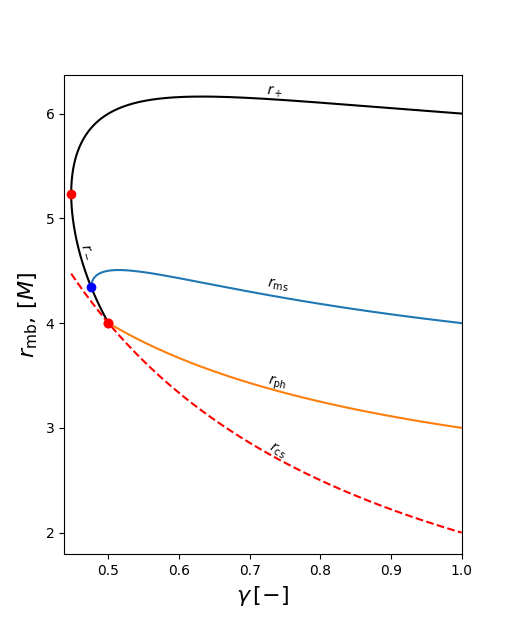
\includegraphics[scale = 0.45]{JNW_orbits.png}
	\captionof{figure}[Характерните орбити за решението на Джанис - Нюман - Уиникър]{\small Характерните орбити за голата сингулярност на Джанис-Нюман-Уиникър при стойности на параметъра $\gamma \in [\frac{1}{\sqrt{5}}, 1]$.}
	\label{JNW_orbits}
\end{minipage}\,\,\,
\begin{minipage}{20em}
Решението на това уравнение, заедно с другите обсъдени орбити са показани на фигура \ref{JNW_orbits}.\\

Виждаме, че решението на уравнение (5.46) съществува само до пресечната му точка с уравнение (5.44). Това е така, понеже под кривата $r_-$, орбитите са стабилни. Стойността на $\gamma$ при която това се случва е $\gamma\approx 0.476$.

\end{minipage}
\newpage
\subsection{Голи сингулярности на Гаус-Боне}
